%%%%%%%%%%%%%%%%%%%%%%%%%%%%%%%%%%%%%%%%%
% Short Sectioned Assignment
% LaTeX Template
% Version 1.0 (5/5/12)
%
% This template has been downloaded from:
% http://www.LaTeXTemplates.com
%
% Original author:
% Frits Wenneker (http://www.howtotex.com)
%
% License:
% CC BY-NC-SA 3.0 (http://creativecommons.org/licenses/by-nc-sa/3.0/)
%
%%%%%%%%%%%%%%%%%%%%%%%%%%%%%%%%%%%%%%%%%

%----------------------------------------------------------------------------------------
%	PACKAGES AND OTHER DOCUMENT CONFIGURATIONS
%----------------------------------------------------------------------------------------

\documentclass[paper=a4, fontsize=11pt]{scrartcl} % A4 paper and 11pt font size

\usepackage[T1]{fontenc} % Use 8-bit encoding that has 256 glyphs
\usepackage{fourier} % Use the Adobe Utopia font for the document - comment this line to return to the LaTeX default
\usepackage[english]{babel} % English language/hyphenation
\usepackage{amsmath,amsfonts,amsthm} % Math packages


\usepackage{marvosym}

\usepackage{tikz}
\usepackage{pgfplots}
\usetikzlibrary{intersections}
\usetikzlibrary{patterns}

\pgfplotsset{compat=1.9}

\usepackage{lipsum} % Used for inserting dummy 'Lorem ipsum' text into the template

\usepackage{sectsty} % Allows customizing section commands
\allsectionsfont{\centering \normalfont\scshape} % Make all sections centered, the default font and small caps

\usepackage{fancyhdr} % Custom headers and footers
\pagestyle{fancyplain} % Makes all pages in the document conform to the custom headers and footers
\fancyhead{} % No page header - if you want one, create it in the same way as the footers below
\fancyfoot[L]{} % Empty left footer
\fancyfoot[C]{} % Empty center footer
\fancyfoot[R]{\thepage} % Page numbering for right footer
\renewcommand{\headrulewidth}{0pt} % Remove header underlines
\renewcommand{\footrulewidth}{0pt} % Remove footer underlines
\setlength{\headheight}{13.6pt} % Customize the height of the header

\numberwithin{equation}{section} % Number equations within sections (i.e. 1.1, 1.2, 2.1, 2.2 instead of 1, 2, 3, 4)
\numberwithin{figure}{section} % Number figures within sections (i.e. 1.1, 1.2, 2.1, 2.2 instead of 1, 2, 3, 4)
\numberwithin{table}{section} % Number tables within sections (i.e. 1.1, 1.2, 2.1, 2.2 instead of 1, 2, 3, 4)

\setlength\parindent{0pt} % Removes all indentation from paragraphs - comment this line for an assignment with lots of text

%----------------------------------------------------------------------------------------
%	TITLE SECTION
%----------------------------------------------------------------------------------------

\newcommand{\horrule}[1]{\rule{\linewidth}{#1}} % Create horizontal rule command with 1 argument of height

\title{	
\normalfont \normalsize 
\textsc{Precalculus \MVAt
 SPS NYU} \\ [25pt] % Your university, school and/or department name(s)
\horrule{0.5pt} \\[0.4cm] % Thin top horizontal rule
\Large Linear Programming Example: Oranges and Grapefruits \\ % The assignment title
\horrule{1pt} \\[0.5cm] % Thick bottom horizontal rule
}

\author{Donatella Delfino} % Your name

\date{\normalsize\today} % Today's date or a custom date

\begin{document}

\maketitle % Print the title

%----------------------------------------------------------------------------------------
%	PROBLEM 1
%----------------------------------------------------------------------------------------

\section{A version of the problem}

A trucker hauls citrus fruit from Florida to Montreal. Each crate of oranges is 4 ft$\,^3$ in volume and weighs 80 lb. Each crate of grapefruit has a volume of 6 ft$\,^3$ and weighs 100 lb. His truck has a maximum capacity of 300 ft$\,^3$ and can carry no more than 6000 lb. Moreover, he is not permitted to carry more crates of grapefruit than crates of oranges. If his profit is \$2.50 on each crate of oranges and \$4 on each crate of grapefruit, how many crates of each fruit should he carry for maximum profit?

{\bf{Solution:}} Set $x$ = number of crates of oranges and $y$ = number of crates of grapefruits. 
\begin{itemize}
\item $x\geq 0,y\geq 0$;
\item The truck has a maximum capacity of 300 ft$\,^3$, so 
\begin{itemize}
\item volume of $x$ crates of oranges + volume of $y$ crates of grapefruits $\leq 300$
\item $\displaystyle 4x+6y\leq 300$.
\end{itemize}
\item The truck can carry no more than 6000 lb so 
\begin{itemize}
\item weight of $x$ crates of oranges + weight of $y$ crates of grapefruits $\leq 6000$
\item $\displaystyle 80x+100y\leq 6000$.
\end{itemize}
\item The truck cannot carry more crates of grapefruit than crates of oranges, so
\begin{itemize}
\item crates of grapefruit $\leq$ crates of oranges
\item $\displaystyle y \leq x$.
\end{itemize}
\end{itemize} 
The system of inequalities is:


\begin{align*} 
\begin{split}
x 	&\geq  0\\
y   &\geq 0\\
4x+6y &\leq 300\\
80x+100y &\leq 6000\\
y&\leq x
\end{split}					
\end{align*}

Graph of the feasible region:

\begin{figure}[htpb]
    \centering
    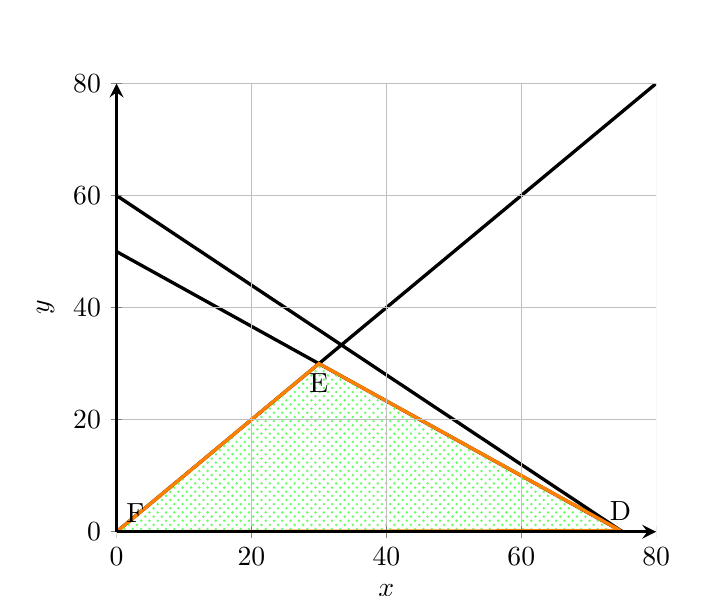
\begin{tikzpicture}
        \begin{axis}[axis on top,smooth,
            axis line style=very thick,
            axis x line=bottom,
            axis y line=left,
            ymin=0,ymax=80,xmin=0,xmax=80,
            xlabel=$x$, ylabel=$y$,grid=major
            ]
            \addplot[name path global=firstline,very thick, domain=0:80]{50-2*x/3};
            \addplot[name path global=secondline,very thick, domain=0:80]{60-(4*x)/5};
            \addplot[name path global=thirdline,very thick, domain=0:80]{x};
            \path[name path=B](0,0) -- (80,0);
\path[name path=C](0,0) -- (0,80);
            \fill[name intersections={of=firstline and secondline,by=point1},
            name intersections={of=firstline and thirdline,by=point2},
            name intersections={of=secondline and thirdline,by=point3},
            name intersections={of=B and secondline,by=point4},
            name intersections={of=C and thirdline,by=point5},
            ][very thick,draw=orange,pattern=crosshatch dots,pattern color=green!60!white](point1)--(point2)--(point5)--(point1);
            \node [above] at (point1) {D};
            \node [below] at (point2) {E};
            \node [above right] at (point5) {F};
            %\addplot[mark=*] coordinates {(0,50)} node[pin=150:{\tiny$80x+100y\leq6000$}]{}
           
        \end{axis}
    \end{tikzpicture}
    
\end{figure}

The corners of the triangle are 
\begin{itemize}
\item $F(0,0)$, which is the intersection of $y=x$, $x=0$ and $y=0$;
\item $E(30,30)$, which is the intersection of $y=x$ and $4x+6y=300$;
\item $D(75,0)$, which is the intersection of $y=0$ and $4x+6y=300$.
\end{itemize}
The profit function is $\displaystyle P=2.5x+4y$. The maximum of $P$ takes place at one of the vertices, so we substitute the coordinates of $D,E,F$ in $P$.

\begin{minipage}{.4\textwidth}
\begin{tabular}{|l|l|l|l|}
\hline
    & $x$ & $y$ & $P$ \\ \hline
$D$ &   0  &   0  &  0   \\ \hline
$E$ &   30  &  30   &  195   \\ \hline
$F$ &   75  &   0  &  187.5   \\ \hline
\end{tabular}
\end{minipage}
\begin{minipage}{.6\textwidth}
The trucker should carry 30 crates of oranges and 30 crates of grapefruits for maximum profit.
\end{minipage}
\section{Another version}
A trucker hauls citrus fruit from Florida to Montreal. Each crate of oranges is 4 ft${}^3$ in volume and weighs 80 lb. Each crate of grapefruit has a volume of 6 ft$\,^3$ and weighs 100 lb. His truck has a maximum capacity of 300 ft$\,^3$ and can carry no more than 6400 lb. Moreover, he is not permitted to carry more crates of grapefruit than crates of oranges. If his profit is \$2.50 on each crate of oranges and \$4 on each crate of grapefruit, how many crates of each fruit should he carry for maximum profit?

 {\bf{Solution:}} Set $x$ = number of crates of oranges and $y$ = number of crates of grapefruits. 
The feasible region is the solution set of the system:

\begin{align*} 
\begin{split}
x 	&\geq  0\\
y   &\geq 0\\
4x+6y &\leq 300\\
80x+100y &\leq 6400\\
y&\leq x
\end{split}					
\end{align*}

Graph of the feasible region:

\begin{figure}[htpb]
    \centering
    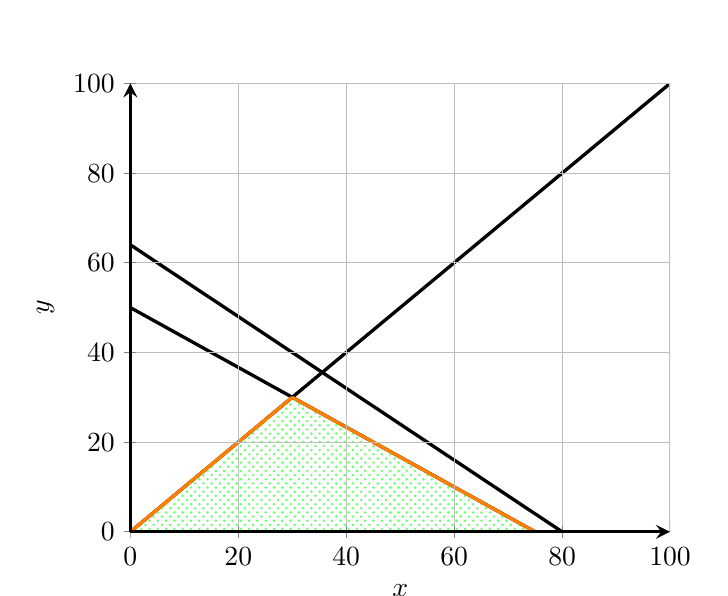
\begin{tikzpicture}
        \begin{axis}[axis on top,smooth,
            axis line style=very thick,
            axis x line=bottom,
            axis y line=left,
            ymin=0,ymax=100,xmin=0,xmax=100,
            xlabel=$x$, ylabel=$y$,grid=major
            ]
            \addplot[name path global=firstline,very thick, domain=0:100]{50-2*x/3};
            \addplot[name path global=secondline,very thick, domain=0:100]{64-(4*x)/5};
            \addplot[name path global=thirdline,very thick, domain=0:100]{x};
            \path[name path=B](0,0) -- (100,0);
\path[name path=C](0,0) -- (0,100);
            \fill[%name intersections={of=firstline and secondline,by=point1},
            name intersections={of=firstline and thirdline,by=point2},
            name intersections={of=secondline and thirdline,by=point3},
            name intersections={of=B and firstline,by=point4},
            name intersections={of=C and thirdline,by=point5},
            ][very thick,draw=orange,pattern=crosshatch dots,pattern color=green!60!white] (point2)--(point4)--(point5)--(point2);
            %\node [above] at (point2) {D};
            %\node [above=0.5cm, left=1.5cm] at (point4) {E};
            %\node [above right] at (point5) {F};
            %\addplot[mark=*] coordinates {(0,50)} node[pin=150:{\tiny$80x+100y\leq6000$}]{}
           
        \end{axis}
    \end{tikzpicture}
    
\end{figure}  

The corners are: $(0,0), (30,30), (75,0)$ and the profit is maximum at $x=30, y=30$.


\end{document}